% !TeX encoding = UTF-8
%综合设计实验报告撰写要求
%标题:1级标题,宋体4号(加粗);
%2级标题,宋体小4号(加粗);
%正文:宋体小4号;
%图号、图名:宋体5号;
%行距:固定行距,20—22;
%图宽度小于1/2正文,放正文边上;
%所有英文及数字的字体采用Times New Roman;

% 设置 zihao = -4 时
% \normalsize = 小四 12pt
% \large = 小三 15pt
\documentclass[UTF8, zihao=-4]{ctexart}
% 中文支持
\usepackage{ctex}
% 代码插入高亮
\usepackage{listings}
% 定义颜色
\usepackage{color}
% 划横线
\usepackage{booktabs}
% 超链接支持
% \usepackage{hyperref}

\usepackage{setspace}
\usepackage{stackengine}

\definecolor{codegreen}{rgb}{0,0.6,0}
\definecolor{codegray}{rgb}{0.5,0.5,0.5}
\definecolor{codepurple}{rgb}{0.58,0,0.82}
\definecolor{backcolour}{rgb}{0.95,0.95,0.92}

\lstdefinestyle{mystyle}{
    backgroundcolor=\color{backcolour},   
    commentstyle=\color{codegreen},
    keywordstyle=\color{magenta},
    numberstyle=\tiny\color{codegray},
    stringstyle=\color{codepurple},
    basicstyle=\footnotesize,
    breakatwhitespace=false,         
    breaklines=true,                 
    captionpos=b,                    
    keepspaces=true,                 
    numbers=left,                    
    numbersep=5pt,                  
    showspaces=false,                
    showstringspaces=false,
    showtabs=false,                  
    tabsize=2
}

\lstset{style=mystyle}
% 设置一个插图存放目录
\graphicspath{{figure/}}

\ctexset {
    % 一级标题
    part = {
        % 默认 \huge\bfseries\centering
        format = \large\bfseries
    },
    % 二级标题
    section = {
        % 默认 \Large\bfseries\centering
        format = \normalsize\bfseries,
    }
}

\begin{document}
    \begin{titlepage} % 封面
        % 居中环境
        \begin{center}
            % 合工大 logo
            
\includegraphics[width=12cm]{cover.png}\\[3cm]
            \textbf{\Huge 电子信息科学与技术综合设计}\\[4cm]
            {\zihao{3}
            \begin{tabular}{ll} 
                设计题目 & \underline{\makebox[10em]{教务数据挖掘与可视化}}  \\
                学生姓名 & \underline{\makebox[10em]{周而良, 裴芝梦}} \\
                学号     & \underline{\makebox[10em]{2013217413, 2013217464}} \\
                专业班级 & \underline{\makebox[10em]{13电信(1)班}} \\
                指导教师 & \underline{\makebox[10em]{xxx}} \\
            \end{tabular} 
            }
            \\[3cm]            
            {\zihao{3} 2016\textasciitilde2017学年第一学期}
            \\[0.5cm]
            {\zihao{4} \today}
        \end{center}
    \end{titlepage}
    
    \tableofcontents % 目录
    \newpage
    
    \part{课题目的}
    电子信息科学与技术综合设计旨在通过学生自主设计与实践,将课本中的理论知识与实践相结合,从而提升学生的专业技能水平。\par
    本次课程设计,我们小组选定的课题为“教务数据挖掘与可视化”,目的是通过设计算法,编写程序对学校教务公开数据进行抓取,然后对数据进行分析与可视化,从普通的数据中提取出有价值的内容。\par
    这个课题需要的知识背景主要涉及到 《概率论与数理统计》、《数据结构》、《计算机网络》、《数据库技术》、《微机原理》、《操作系统》等课程。同时额外的涉及到了代码版本控制、Python 编程语言、异步编程、文档型数据库、缓存技术、数据向量化,可视化等方面的专业知识。能够训练我们在软件开发,高性能爬虫,数据挖掘,数据可视化等方向的专业素养。
    \part{课题任务}
    \begin{enumerate}
        \item 教务公共接口分析\\
            使用个人账号登录教务系统,分析教务提供了哪些服务接口,包括接口的地址、请求方式、请求参数、身份的验证、返回的数据内容等。用来确定最终我们能得到的数据内容、格式以及爬虫对页面的访问顺序。
        \item 基本架构\\
            在完成‘教务公共接口分析’任务后,根据我们的需求做合理的技术选型,确定需要何种编程语言与框架、何种数据库、数据库结构、爬虫算法。
        \item 页面数据序列化模块编写\\
            完成了整体的设计,程序实现的第一步就是对网页中人眼可识别的、被修饰渲染的页面数据转换为程序可识别、可处理、可分析的格式化数据。
        \item 高性能爬虫实现\\
            庞大的数据量与个人电脑性能高度的不对等决定了我们需要运用各种技术实现对爬虫进行高性能的实现。数据的抓取是一个非常耗时的工作,任何一个小的遗漏都会导致性能的急剧损失,同时,也需要完善的测试避免程序的出错终止或是数据的丢失。
        \item 数据结果统计与简单分析\\
            对抓取的格式化数据进行分析,从普通的数据中提取出有价值的内容,研究得到的数据可产生的实际应用。
    \end{enumerate}
    
    \part{课题内容}
    \section{教务公共接口分析}
    网页内容的传输是建立在超文本传输协议协议上的,超文本传输协议(英文:HyperText Transfer Protocol,缩写:HTTP)是互联网上应用最为广泛的一种网络协议。设计HTTP最初的目的是为了提供一种发布和接收HTML页面的方法。通过HTTP或者HTTPS协议请求的资源由统一资源标识符(Uniform Resource Identifiers,URI)来标识。\cite{wiki:Hypertext_Transfer_Protocol}\par
    
    HTTP/1.1协议中共定义了八种方法(也叫“动作”)来以不同方式操作指定的资源:
        
    \begin{description}
        \item[OPTIONS:] 这个方法可使服务器传回该资源所支持的所有HTTP请求方法。用'*'来代替资源名称,向Web服务器发送OPTIONS请求,可以测试服务器功能是否正常运作。
        \item[HEAD:] 与GET方法一样,都是向服务器发出指定资源的请求。只不过服务器将不传回资源的本文部分。它的好处在于,使用这个方法可以在不必传输全部内容的情况下,就可以获取其中“关于该资源的信息”(元信息或称元数据)。
        \item[GET:] 向指定的资源发出“显示”请求。使用GET方法应该只用在读取数据,而不应当被用于产生“副作用”的操作中,例如在Web Application中。其中一个原因是GET可能会被网络蜘蛛等随意访问。
        \item[POST:] 向指定资源提交数据,请求服务器进行处理(例如提交表单或者上传文件)。数据被包含在请求本文中。这个请求可能会创建新的资源或修改现有资源,或二者皆有。
        \item[PUT:] 向指定资源位置上传其最新内容。
        \item[DELETE:] 请求服务器删除Request-URI所标识的资源。
        \item[TRACE:] 回显服务器收到的请求,主要用于测试或诊断。
        \item[CONNECT:] HTTP/1.1协议中预留给能够将连接改为管道方式的代理服务器。通常用于SSL加密服务器的链接(经由非加密的HTTP代理服务器)。
    \end{description}

    方法名称是区分大小写的。当某个请求所针对的资源不支持对应的请求方法的时候,服务器应当返回状态码405(Method Not Allowed),当服务器不认识或者不支持对应的请求方法的时候,应当返回状态码501(Not Implemented)。\par
    HTTP服务器至少应该实现GET和HEAD方法,其他方法都是可选的。当然,所有的方法支持的实现都应当匹配下述的方法各自的语义定义。此外,除了上述方法,特定的HTTP服务器还能够扩展自定义的方法。例如:
PATCH(由 RFC 5789 指定的方法):用于将局部修改应用到资源。\par
    具体问题具体分析,对于教务系统来说,进入教务系统的第一步就是登录页面,只有登录后我们才能对接口进一步的分析。\par
    
    \begin{figure}
        \centering
        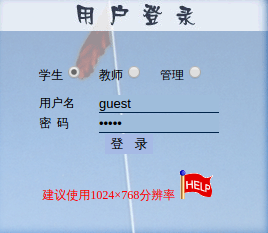
\includegraphics[width=0.5\linewidth]{figure/interface-login}
        \caption{登录页面}
        \label{fig:interface-login}
    \end{figure}
    
    进入教务系统后,其主要的公共数据查询菜单只要集中在“课程信息”一栏,除去个人课表一栏,主要的数据获取来源为“计划查询”与“课程查询”功能。\par
    
    \begin{figure}
        \centering
        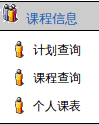
\includegraphics[width=0.5\linewidth]{figure/interface-menu}
        \caption{功能菜单}
        \label{fig:interface-menu}
    \end{figure}
    
    在计划查询页面中, 我们可以查询每个专业的学期课程计划与,任选课,实际上每个学期任选课是全校通用的,意味着抓取时我们每个学期只需请求一次选修课计划即可。\par
    
    \begin{figure}
        \centering
        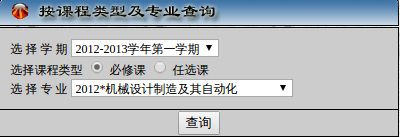
\includegraphics[width=0.5\linewidth]{figure/interface-plan}
        \caption{计划查询页面}
        \label{fig:interface-plan}
    \end{figure}
    
    在计划查询的结果页面,我们可以得到该学期专业的课程数据,包括“课程代码”,“课程名称”,“学分”,“学时”,“开课单位”五个字段,从数据库建建模的角度来说,这几个字段应当是一门课程的属性,虽然有不同专业不同学期的计划,但实际上是可以把相应的课程归为一个,然后在计划表中添加计划即可。\par

    \begin{figure}
        \centering
        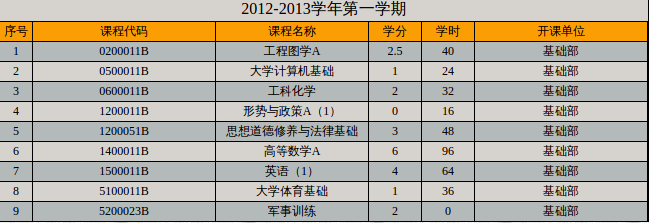
\includegraphics[width=0.5\linewidth]{figure/interface-plan-result}
        \caption{计划查询结果页面}
        \label{fig:interface-plan-result}
    \end{figure}
    
    在课程查询页面,我们可以通过课程代码或者课程名称来查询指定的教学班,然后再点击对应班的课程代码获得教学班详情。再根据对应的学期代码,课程代码,教学班号查询到每个班的学生。
    
    \begin{figure}
        \centering
        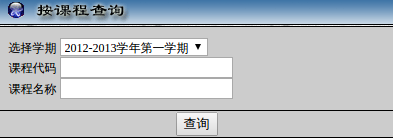
\includegraphics[width=0.5\linewidth]{figure/interface-search-course}
        \caption{课程教学班搜索页面}
        \label{fig:interface-search-course}
    \end{figure}
    
    \begin{figure}
        \centering
        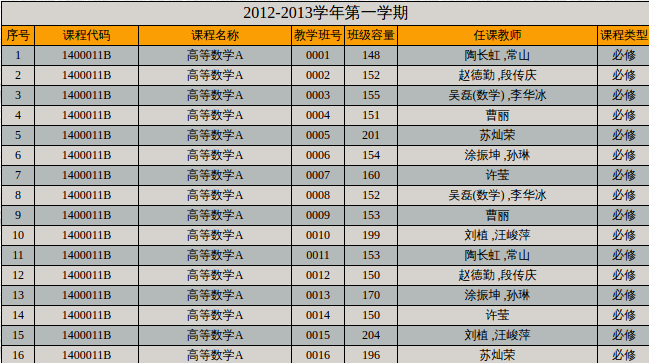
\includegraphics[width=0.5\linewidth]{figure/interface-search-result}
        \caption{课程教学班搜索页面}
        \label{fig:interface-search-result}
    \end{figure}
    
    \begin{figure}
        \centering
        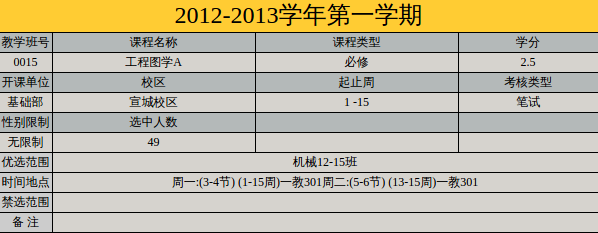
\includegraphics[width=0.5\linewidth]{figure/interface-class-info}
        \caption{教学班详情页面}
        \label{fig:interface-class-info}
    \end{figure}

    最终,经过不断地尝试与发掘后, 我们的爬虫最终需要用到的有登录,计划查询,课程查询,教学班信息查询,教学班学生查询这五个功能。
    
    \section{基本架构}
    
    我们的主力开发语言是Python,Python语言简洁优雅,在Web开发,科学计算,机器学习,数据挖掘方向都有很成功的应用。经过之前接口的分析,我们初步设计了如下的爬虫页面抓取流程:
    
    \begin{figure}
        \centering
        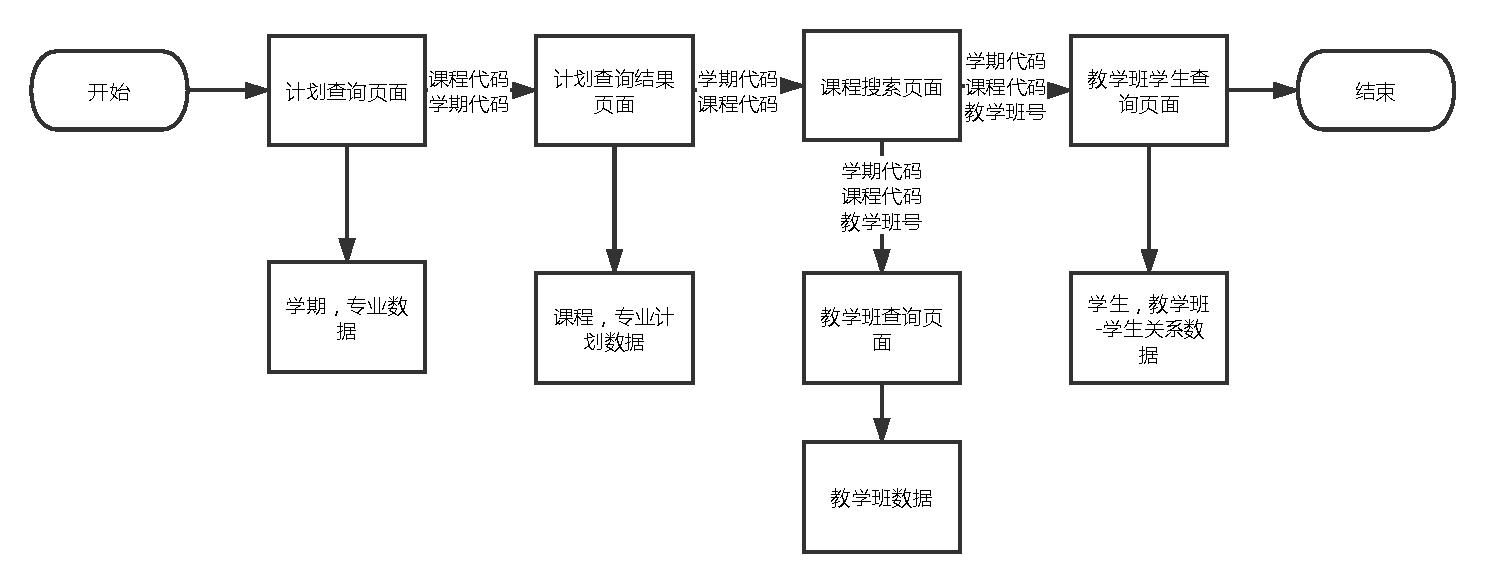
\includegraphics[width=1.0\linewidth]{figure/seq1}
        \caption{爬虫页面抓取流程}
        \label{fig:seq1}
    \end{figure}
    
    其主干是各个页面的访问顺序,同时传递给下一个访问页面的参数,分支则是从该页面获取到的数据。表面上看,各个页面是顺序访问,但是实际上每个页面都会产生大量的参数传递到下一层,也就是说,实际运行起来的效果类似于一个\textbf{多叉树},这就导致了页面的请求数量是呈几何倍数的增长,更为严重的是,越后面的请求返回的数据量反而更大,进一步加剧了这个问题。如何设计高效,合理,稳定的爬虫算法显得格外重要了。
    
    \section{数据库模型}
    经过对公开数据接口的挖掘,以及对教务数据结构的分析,我们决定将数据分为“学期”,“专业”,“课程”,“专业计划”,“教学班”,“学生”六张表储存主要数据以及一张“教学班-学生”关系表储存多多对关系。对于数据库模型,我们除了考虑到如何储存技术之外,还涉及到了程序对数据的操作与表达能力。我们使用了\textbf{对象关系映射}技术作为代码与数据之间的中间件,对象关系映射(英语:Object Relational Mapping,简称ORM,或O/RM,或O/R mapping),是一种程序设计技术,用于实现面向对象编程语言里不同类型系统的数据之间的转换。从效果上说,它其实是创建了一个可在编程语言里使用的“虚拟对象数据库”。面向对象是从软件工程基本原则(如耦合、聚合、封装)的基础上发展起来的,而关系数据库则是从数学理论发展而来的,两套理论存在显著的区别。为了解决这个不匹配的现象,对象关系映射技术应运而生。
    简单的说:ORM相当于中继数据。\cite{wiki:Object-relational_mapping}
    
    Python ORM框架中比较SQLAlchemy和Django ORM,后者实际上是作为其Web开发框架的一个部分,在数据描述,校验及数据库迁移方面都更加便利,另外我们后期也可以无需修改便可将其利用到教务数据相关的Web应用当中,我们的数据模型类原型如下:
    
    \lstinputlisting[language=Python]{code/models.py}
    
    \section{页面数据序列化模块编写}
    前面对数据库模型的设计及对象关系映射技术的使用将原始的数据库数据库数据转换成了可操作的代码对象,那么相应的,我们也需要通过一定的方式对教务的页面进行解析,抽取出其中有用的数据,变成可操作可导出的序列化数据,这也是爬虫最基本的逻辑。而这部分工作对于我们这次课题却是最繁重却又不是最复杂的部分。好在我组周而良同学在一年前就展开了相关工作,开发出了功能丰富,配置灵活的框架,其Github上的特性介绍\cite{er1iang/hfut}如下:
    
    \begin{itemize}
        \item 同时支持合肥校区和宣城校区的教务系统, 对应接口的使用方式完全相同
        \item 支持会话自动更新, 无需担心超过时间后访问接口会出错
        \item 支持非法参数检查, 你再也不用担心一不小心就被封了 IP 了
        \item 支持全局配置 HTML 解析器, 同时照顾了不会处理依赖编译的新手和对性能有要求的场景
        \item 使用简单, 只需声明一个  ``hfut.Student``  对象即可调用所有接口
        \item 接口丰富, 提供了所有学生能够使用的教务接口, 除此外还有正常情况下学生无法访问到的接口
        \item 可以灵活控制课表数据, 再也不需要各类上传个人隐私, 功能臃肿的课表软件了
        \item 数据能够轻松导出, 能够为基于工大教务数据的服务或应用提供强大的底层支持
        \item 提供了强大的选课功能, 你能轻松查询可选的课程, 查看教学班级选中人数, 批量提交增删课程数据
        \item 对开发友好, 每个接口返回的数据结构都提供了描述, 同时提供了用于继承的基类以及页面处理的函数和其他工具提升你的开发效率
        \item Python2/3 兼容, 代码在 2.7,3.3,3.4,3.5, pypy 五个版本上进行了测试
    \end{itemize}
    
    其完整的实现省去了我们很多的精力,也算是对本次课题的提前准备。有了这个模块的支持,教务功能的访问只要简单几行代码就能实现。以我们本次课题所需要访问的接口为例,访问我们需要的接口只要以下几个调用即可。
    
    \begin{lstlisting}[language=Python]
    from hfut import Student
    s = Student(学号, 密码, 校区)
    # 获取专业和学期
    s.get_code()
    # 获取教学计划
    s.get_teaching_plan(xqdm=学期代码, zydm=专业代码)
    # 获取课程教学班
    s.search_course(xqdm=学期代码, kcdm=课程代码)
    # 获取教学班详情
    s.get_class_info(xqdm=学期代码, kcdm=课程代码, jxbh=教学班号)
    # 获取教学班
    s.get_class_students(xqdm=学期代码, kcdm=课程代码, jxbh=教学班号)
    \end{lstlisting}
    
    \section{高性能爬虫实现}
    
    这里的爬虫实现,实际上是对前面所做工作的整合,但这确是整个课题最复杂,最重要的一个部分,这就相当于一个流水线,各个部分的机器已经设计并制造成功,现在需要一个调度中心对整个流水线进行调度使之效率达到最高。我们刚开始想的是简化工作,使用Scrapy框架来完成爬虫的设计,Scrapy是一个非常成熟的框架,它基于事件驱动的异步网络框架Twisted,将爬虫工作分解为“发送请求”,“响应解析”,“序列化数据处理”三个部分,然后使用内置的引擎进行调度。其数据流模型全都是围绕着这个引擎工作的。\cite{scrapy_architecture_overview}\par
    我们也尝试了使用框架实现了我们的爬虫,但是不幸的是效果非常的差,究其原因,正是我们之前提到的,多叉树导致的请求数放大,而且数据量大的教学班学生数据和教学班学生关系数据请求放在最后,这些数据单个条目数据量不大但数据记录数量非常的多,而Scrapy中的数据记录只能一个个生成然后再等待调度。这让整个程序完全将资源消耗在完全可以避免的任务调度上而不是页面的抓取工作。加之Python的GIL问题,程序只能在单个CPU核心运行,完全没用有效地利用系统资源,为此我们决定自行设计和编写爬虫调度程序。\par
    
    \begin{figure}
        \centering
        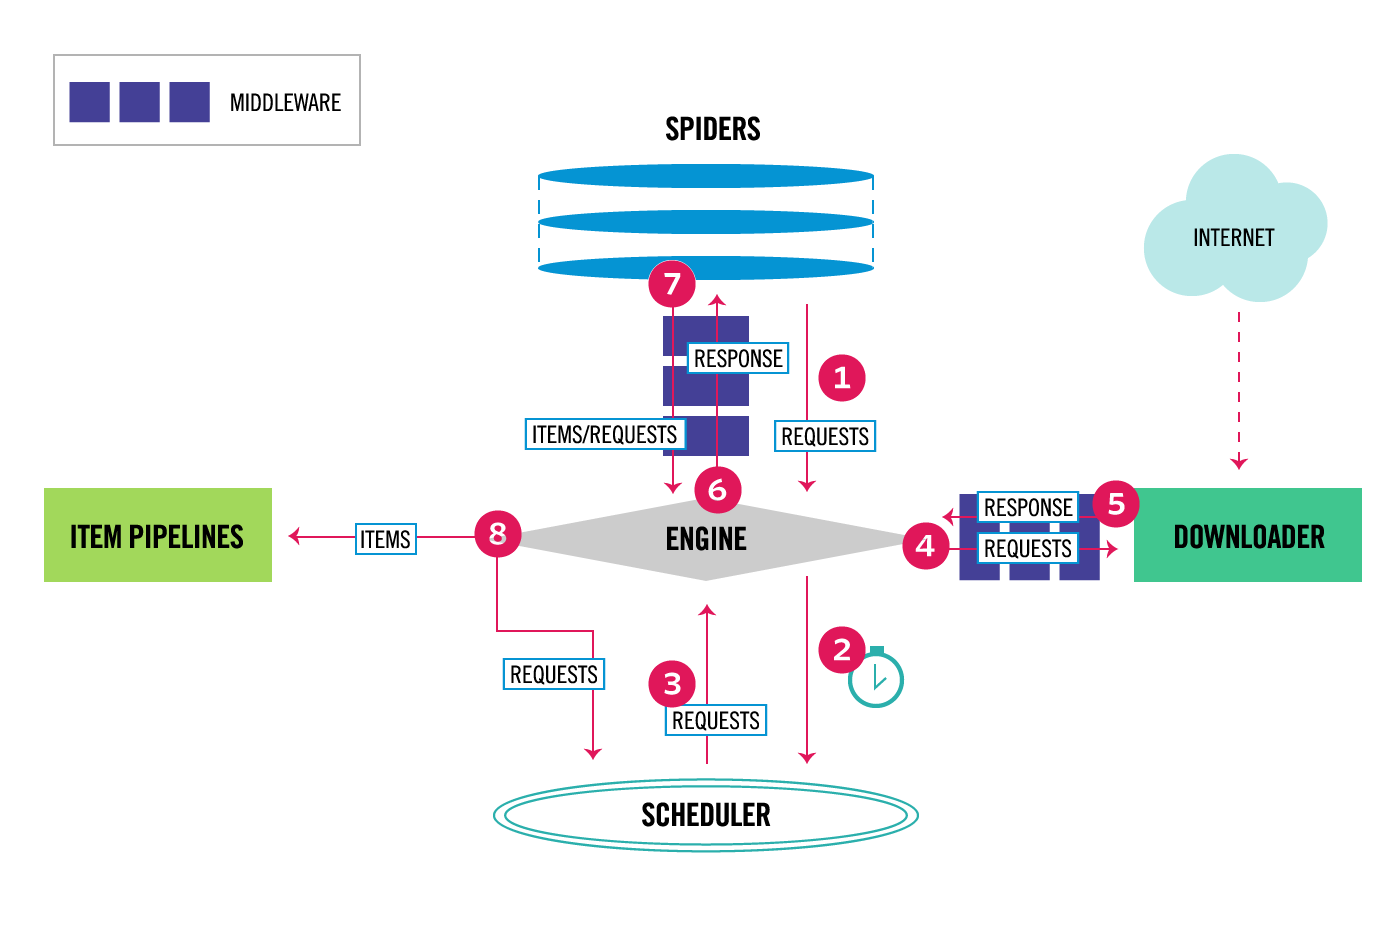
\includegraphics[width=1.0\linewidth]{figure/scrapy_architecture}
        \caption{Scrapy架构}
        \label{fig:scrapy_architecture}
    \end{figure}
    
    高性能爬虫实现的核心就是冲利用操作系统任务调度分片的机制,将任务处于IO阻塞态时自动切换到其他任务达到并发的效果。还是由于之前提到的Python的GIL问题,我们不使用Python标准库自带的线程实现而使用Gevent这个基于libev的协程框架。它底层是使用C语言实现,绕过了Python的语言限制,能够充分的利用多核。除此之外,我们取代了之前的SQL数据库而使用NoSQL数据库(Mongodb),在内存中建立索引后能极大地提升性能。
    刚开始,我们仿照Scrapy的设计,将实现了很细的任务细粒度,结果就是我们自行设计的任务调度程序也和使用Scrapy框架是一样,CPU跑满,整个程序将大量的时间花费在了任务调度上,不仅没有利用到网络IO的等待时间,反而导致请求任务一直处于等待状态。\par
    我们按照架构中的流程[\ref{fig:seq1}]重新设计任务单元,使用了两个任务池来,一个任务池负责页面的访问与解析,同时将数据库记录请求提交到数据库任务池,这样就将IO和资源的消耗分成了两个部分,可以分别对其进行优化。\par
    对于页面请求解析的任务池,我们知道,各个页面的访问是有先后顺序的,但是对于一个任务池来说,其每个任务之间的关系是平行的,对于某一个任务,我如何获取到它执行所需要的参数,又如何将运行的结果传递到下一个任务呢?答案就是树的遍历过程,我们前面讲到我们请求的过程类似与一棵树,我们可以通过递归来遍历每个任务,然后将返回的参数作为下一个任务的参数。其核心实现如下:

    \lstinputlisting[language=Python]{code/dfs.py}
    
    \verb|dispatch|函数就是递归逻辑,他从\verb|step|参数从获取当前需要执行的任务,从\verb|args|参数获取这个任务所需要的参数,执行这个任务,如果任务返回了下一个任务的参数,便将其提交到任务池进行下一步。简单的几步构成了页面请求解析任务分配工作的核心,运行效率非常高。不过在实际运行中我们发现,当并发数量太大,导致教务系统出错无法得到我们想要的结果,我们必须任务池的并发进行限制,但Gevent池的实现在控制任务并发时使用的不是可重入锁,导致当任务池大小不够,任务递归的获取锁导致程序死锁,为解决这个问题我们使用了一个队列,将深度优先搜索改为了广度优先搜索。这样任务的不再递归提交,消除了死锁。

    \lstinputlisting[language=Python]{code/bfs.py}  
       
    对于数据库请求的任务池,我们充分利用Mongodb的特性,首先就是仅在记录不存在时插入,这在传统SQL数据库中必须执行两次命令,而Mongodb只需一条命令,本来NoSQL写入性能就好,加之Mongodb的索引完全建立在内存当中,查询速度非常的快。\par
    为了避免每一个数据库请求就发送一次消息,在这里我们设计了批量写入的算法,仅当数据库请求达到一定量时才进行一次发送,最后在页面请求解析任务全部完成后,对剩余的不够数目的请求统一进行处理,再一次的提升了性能。

    \lstinputlisting[language=Python]{code/db_manager.py} 
    
    \section{数据分析}
    
    以学生数据为例,我们共获得整个校区13567个学生的学号、姓名与性别,我们经过代码统计得到下表:
    
    \begin{table}[htbp]
        \centering
        \begin{tabular}{ccccc}
            \toprule
            入学年份 &女&	男&	比例&	合计\\
            \midrule
            2012&	586&	2037&	3.476109&	2623\\
            2013&	604&	2332&	3.860927&	2936\\
            2014&	590&	2412&	4.088136&	3002\\
            2015&	650&	2346&	3.609231&	2996\\
            2016&	459&	1551&	3.379085&	2010\\
        \end{tabular}
        \caption{宣城校区历年人数统计及男女比例}
    \end{table}
    
    我们很容易就发现,2012-2015年招生人数逐步上涨,但今年却回落了很多,同时,部分理工专业的取消,商务英语专业的增设,校区男女比例下降很多,与实际事实相符,利用统计图来表现则为图\ref{fig:sex_plot}效果。
    
    \begin{figure}
        \centering
        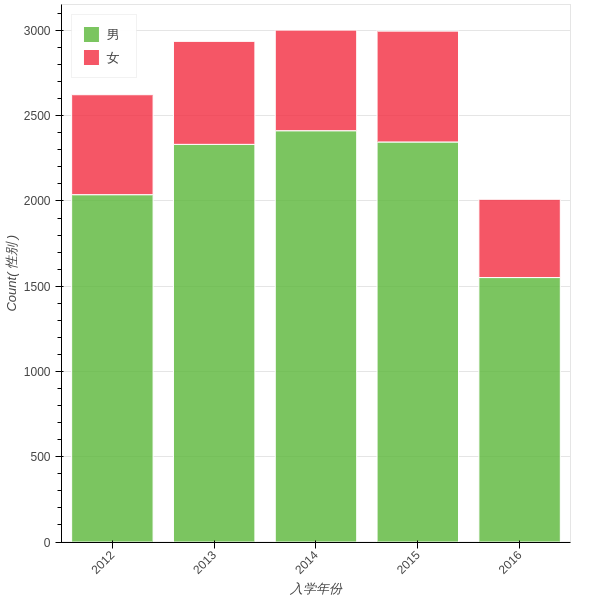
\includegraphics[width=0.7\linewidth]{figure/sex_plot}
        \caption{宣城校区历年人数统计及男女比例}
        \label{fig:sex_plot}
    \end{figure}
    
    另外,还实现了对任意学生各学期课程的查询,由于不方便在报告中展示其动态效果,我们会将整个课题报告与代码同步到 https://github.com 供有兴趣的读者进行研究。
    
    \part{课题结果}
    \section{代码工作量统计}
    
    我们使用Linux下的wc和find命令相结合,统计了本次课题主要的代码文件代码行数,这不包括一些日志代码,简单的脚本和最终的数据分析程序。最终得出的数据以行数为单位。
    
    \begin{table}[htbp]
        \centering
        \begin{tabular}{ccccccc}
            \toprule
            \multicolumn{5}{c}{爬虫完整代码} \\
            \cmidrule{1-5}
            数据模型 & 爬虫原型 & 任务调度 & 爬虫任务 & 测试 & 接口模块 & 总计 \\
            \midrule
            90      & 532      & 94      & 143      & 79  & 1952     & 2890  \\
            \bottomrule
        \end{tabular}
        \caption{主要代码行数统计}
    \end{table}
    
    \section{数据库记录统计}
    
    \begin{table}[htbp]
        \centering
        \begin{tabular}{cccccccc}
            \toprule
            term & major & course & plan & class & student & class\_student & 总计  \\
            \midrule
            10   & 120   & 1231   & 2201 & 10013 & 13567   & 822919        & 850061 \\
            \bottomrule
        \end{tabular}
        \caption{数据库各张表记录数统计}
    \end{table}
    
    \section{总结}
    本次课题我们从课本所学出发,以同学们熟悉的教务系统作为案例,利用了众多技术与算法,完成了从接口分析,数据模型建立,再到高性能爬虫实现及数据分析,极大地提升了我们在数据科学方向的专业能力。当然,
    本次课题我们虽然出色的完成了对数据抓取工作,但是数据分析和可视化工作因时间原因只研究了一部分,实际上我们还可以利用这些数据挖掘出更多有趣的信息,后期再抽出时间对这次的数据做更多维度的分析与应用。\par
    另外,我们还要对代码进行整理并发布,为之后对其他一些校区数据研究课题提供参考。
    
%文献引用
\bibliographystyle{unsrt}
\bibliography{reference}    

\end{document}

